\documentclass[letterpaper, 11pt]{article}
\usepackage{amsmath}
\usepackage{amssymb}
\usepackage{float}
\usepackage{inputenc}
\usepackage[left=2cm, right=2cm, top=2cm, bottom=2cm]{geometry}
\usepackage{graphicx}
\usepackage{float}
\usepackage{caption}
\usepackage{extarrows}
\usepackage{xcolor}
\usepackage{lscape}
\usepackage{pdflscape}
\usepackage{pdfpages}
\usepackage{multicol}
\usepackage{leftindex}
\usepackage{algorithm2e}
\SetKwComment{Comment}{/* }{ */}
%\RestyleAlgo{ruled}
\usepackage{mathtools}
\usepackage{hyperref}
\hypersetup{
    colorlinks=false,
    }

% Listings
\usepackage{listings}
\usepackage{color}
\input{lst_style.tex}

% NewCommands
\newcommand{\peq}{ \mathrel{+}= }
\newcommand{\muleq}{ \mathrel{*}= }
\newcommand{\sign}{ \text{sign}}
\newcommand{\bm}[1]{\begin{bmatrix} #1 \end{bmatrix}}
\newcommand{\lx}[2]{\leftindex #1 {#2}}
\newcommand{\norm}[1]{\left\lvert #1 \right\rvert}
\newcommand{\itbf}[1]{\textit{\textbf{#1}}}
\newcommand{\mdet}[1]{\norm{\begin{matrix} #1 \end{matrix}}}



\title{Parametric Model Identification for Motor-Propeller Actuator Dynamics}
\author{Sesha N. Charla}
\date{\today}


\begin{document}
\maketitle
\tableofcontents

%===============================================================================
\newpage
\section{RPM Measurement}
An is interrupt triggered for every commutation high and the ISR gets the counter
value of an independently runing timer. Using this value, the RPM is calcluated
at every interrupt trigger as follows:
\begin{align*}
    rpm &= \frac{60 f_t}{N_p \times T_c}\\
    \text{Where,} \qquad &\\
    f_t &- \text{Frequency of the timer counts (here, $1$ MHz)}\\
    N_p &- \text{Number of pole-pairs in the BLDC motor (here, $7$)}\\
    T_c &- \text{Timer counts between the two interrupts}
\end{align*}

The above method of measurement is verified against the tach-meter reading. The
readings are in agreement with each other, validating the measurement method.
\begin{figure}[H]
    \centering
    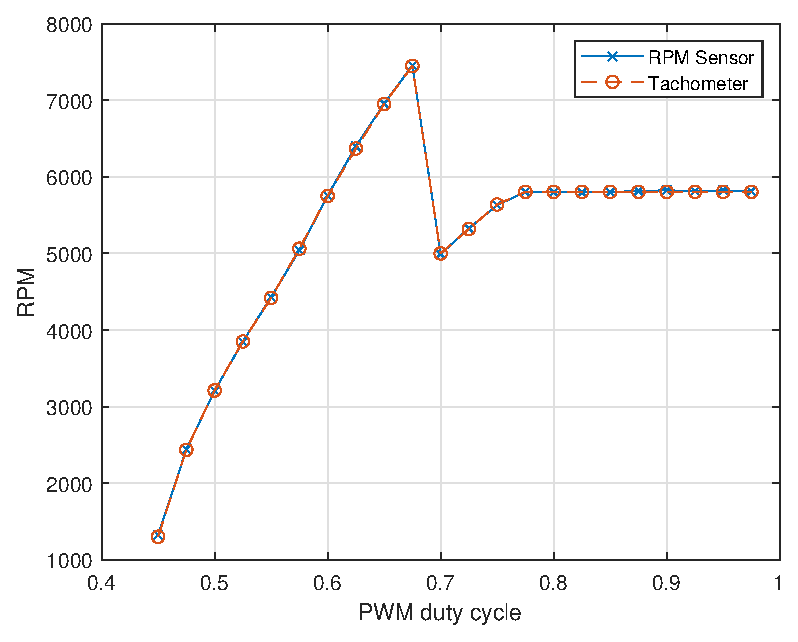
\includegraphics[width=0.5\textwidth]{./figs/rpm_feedback/static_calib.eps}
    \caption{Rpm sensor and tachometer readings}
\end{figure}

The above method has an inherent flow at very low $rpm$s where there is no
commutation at a given sampling instance which results in a zero rpm at that
sample making the sensor noisy. This can be avoided by holding the rpm value
from the previous measurement if there is no commutation in the sample instance.

\bigskip

\itbf{Using external interrupt and  timer}
\par The commutations can be counted using external interrupts. The actual measurement of rpm involves a raising-edge triggered external interrupt and a timer interrupt. The ISR of the external interrupt updates a counter corresponding to the pulses (here, the electrical commutations). The timer-interrupt polls for this counter value at the specified frequency $(f_s)$ and resets the counter. The rpm is calculated from this counter value as follows:
$$rpm = \frac{counter\_value}{N_P} \times f_s \times 60$$
where, \\
$N_p - $ No. poles in the BLDC motor\\

\par The minimum rpm that can be measured depends on the sampling frequency and the poles in the BLDC motor $(= \frac{60f_s}{N_P} )$. And the maximum depends on the clock frequency of the micro-controller as the frequency of interrupts and ISR calls becomes the bottleneck in this case. The resolution of the sensor also depends on the sampling frequency and poles as the counter value is an integer. We have,
$$Sensor \, resolution = \frac{60f_s}{N_P}$$

\par For the current system the range of rpm is $[2000, 10000]$. The number of poles in BLDC motor are $12$. Assuming the acquisition frequency of $400\,Hz$, the resolution for the above sensor will be:
$$Sensor \, resolution = \frac{60f_s}{N_P} = 2000 \, rpm = 209.4395 \, rad/s$$
For $100 \, Hz$ acquisition rate:
$$Sensor \, resolution = 500 \, rpm = 52.3599 \, rad/s$$

\par The main source of sensor noise in this case is the latency of the external interrupt. The counter value will be oscillating around the actual value based on the timing of external and timer interrupts causing the measured rpm to fluctuate. Based on the resolution calculations above, the signal-to-noise ratio of the system will be very high if the current implementation is used. \\

\par This problem of resolution and signal-to-noise ratio is due to the interfacing method used. Alternatively, the following method is propsoed to overcome this problem.

\bigskip

\itbf{Using two timers and an external interrupt}
\par We use and additional timer as a high frequency counter of frequency $f_t$ for calculating the rpm at every sampling period as follows:
$$rpm = \frac{counter\_value \times f_t}{N_P \times time\_counts} \times 60$$
where, \\
$N_p - $ No. poles in the BLDC motor\\
$time\_counts - $ Number of timer interrupt counts during the sampling interval.\\
Hence, we have, maximum number of $time\_counts$ in a sampling interval is $f_s/f_t$\\
$$\implies Sensor \, resolution = \frac{60f_s}{N_P f_t} = rpm_{min}$$
Therefore, the resolution of the sensor can be increased by arbitrarily increasing the frequency of the high frequency counter, limited only by the hardware.\\

For example, if $f_h = 1000\, Hz$, for the same values as above, the resolution of the sensor:
$$Sensor \, resolution = \frac{60f_s}{N_P \times f_t} = \frac{2000}{1000} = 2 \, rpm = \frac{1}{\pi} \, rad/s$$

\par This method will reduce the signal-to-noise ratio significantly.

\subsection{Measurement Algorithm}
\par In higher rpm cases there are more than one measurement instance wthin
the sample time. Median of these measurements can be used to reduce sudden spikes in the data due to interrupts skips. Combining this with
higher resolution algorithm, we have the algorithm for rpm measurement:\\

Let $C_c$ be the current value of the 32-bit timer, $P_c$ the previous value and $n_C$ be the number of commutations within the sample.\\

At every interrupt trigger (in ISR)

    \begin{algorithm}[H]
        $n_C \peq 1$\;
        $\delta t_k = C_c - P_c$\;
        \If{ $\delta t_k \leq 0$ }
            {$\delta t_k \peq 2^{32}$ \Comment*[r]{Correcting for integer overflow}}
        $\pmb{\delta t_k} [n_C-1] =  \delta t_k$\;
        $P_c = C_c$\;
    \end{algorithm}

At every sampling instance (in $get\_rpm()$):

    \begin{algorithm}[H]
        $N_p = 7$\;
        $f_t = 10^6$\;
        $M = \frac{2 \pi}{N_p} \times f_t$\;
        \eIf {$n_C > 0$ and $n_C \leq n_{C_{max}}$ and $\norm{n_C - n_{C_{old}}} \leq \delta n_{C_{max}}$}
            {$\omega = \frac{M}{\text{Median}(\pmb{\delta t_k})}$ \Comment*[r]{Median removes spikes in the data}
             $ \omega_{old} = \omega$\;
             $n_{C_{old}} = n_C$\;
            }
             {$\omega = \omega_{old}$}
        $n_C = 0$\;
        $\pmb{\delta t_k} = \pmb 0$\;
    \end{algorithm}

\begin{figure}[H]
    \begin{minipage}{0.49\textwidth}
        \begin{figure}[H]
            \centering
            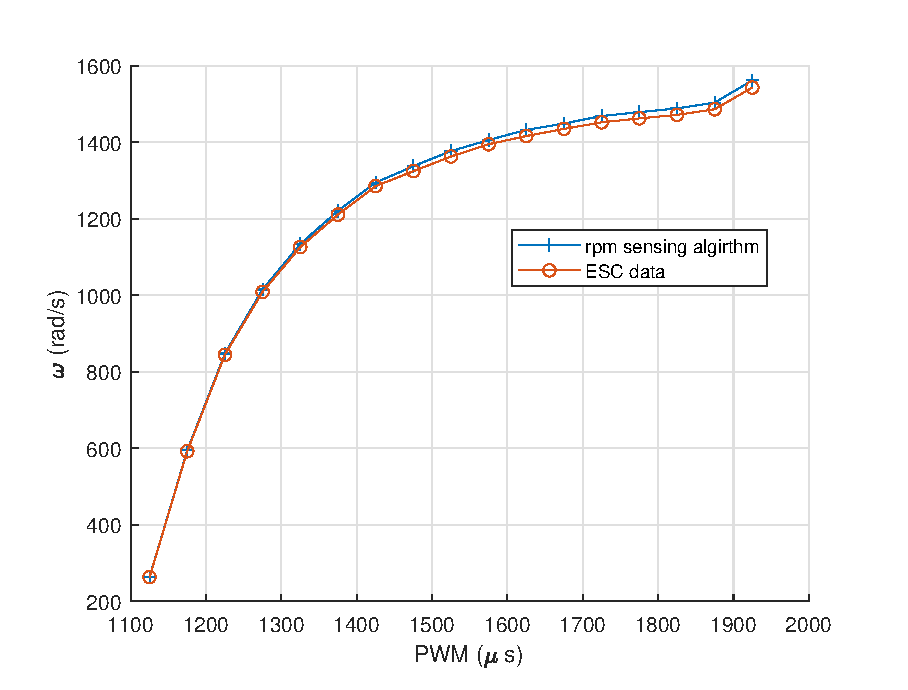
\includegraphics[width = \textwidth]{./figs/rpm_feedback/rpm_meas_noprop.eps}
            \caption*{Without Propeller}
        \end{figure}
    \end{minipage}
    \begin{minipage}{0.49\textwidth}
        \begin{figure}[H]
            \centering
            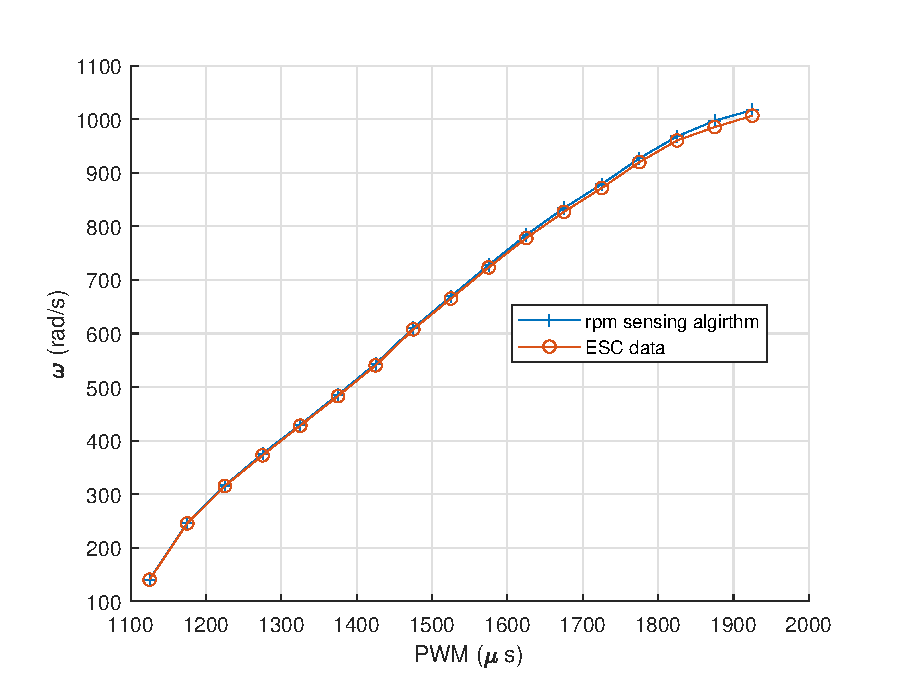
\includegraphics[width = \textwidth]{./figs/rpm_feedback/rpm_meas_prop.eps}
            \caption*{With Propeller}
        \end{figure}
    \end{minipage}
    \caption{Validating the measurement algorithm}
\end{figure}

%===============================================================================
\newpage
\section{BLDC Motor Model and Static Calibration}
\subsection{ESC and non-linear input compensation}

The castle creations ESC has a micro-controller that non-lineraly scales the input PWM signal's duty-cycle to the duty-cycle of the $24\,kHz -$PWM signals to the inverter effectively scaling the source voltage to the motor by the duty-cycle. This is done to have a linear input to thrust curve instead of a quadratic one.

The input transmission can be described as follows: The $400\,Hz-$PWM duty cycle ($u_p$) islineraly scaled to a throttle ratio $(p)$ ($\%$ power-out) between 0 and 1. Which is then filters using a non-linear function $(g_u)$ to get the PWM duty-cycle input to the inverter ($u$) \cite{kim2017electric}.

\begin{align*}
    u_p \rightarrow \boxed{g_u(.)} \rightarrow u
\end{align*}
and finally,
$$V_s = u V_{in} \qquad u \in [0, 1]$$

$u$ is considered as the input to the motor-propeller system and the necessary invertion will be performed for transmitting the signals.

\itbf{Scaling PWM Singal Duty cycle based on switching frequency}
Pixhawk-4 uses a switching frequency of $400\,Hz$ for its PWM signals (can be swithed to $50 \, Hz$ which is not that usefull in case of BLDC motors but usefull for servos). The controller thus scales the PWM duty cycle to the duration of on-time of the signal in its period in 'microseconds'. These inputs are handelled as integer types within the range [800, 2200]\cite{px4_pwm}.

The current ESC that has the rpm-feedback capabilites has an operating range between $1110 \, \mu s$ and $1890 \, \mu s$. After that, the ESC switchs to a constant power mode which sets the rpm to a constant.
\begin{align*}
    \text{Period of the PWM wave } &= \frac{1}{400} \times 10^6 \, \mu s = 2500 \, \mu s\\
    \text{Minimum Operating Duty Cycle } &= \frac{1110}{2500} = 0.444\\
    \text{Maximum Operating Duty Cycle } &= \frac{1890}{2500} = 0.756\\
\end{align*}

$u$ can be considered to be the actual input to the system and system identification with the propeller. It turns out that the parameters of the above non-linear filter are not estimatable with the give information. To solve this problem, we chose normalized no-load angular velocity of the motor as the input instead.

\subsection{Normalized No-load Angular Velocity Input}

We have the no-load dynamic model for the BLDC motor:
\begin{align*}
    J_m \dot \omega_m + (K_r K_v  + b_f) \omega_m + M_f &= u K_r V_{in}
\end{align*}
At steady state ($\dot \omega_m = 0$), the above equation becomes:
\begin{align*}
    (K_r K_v  + b_f) \omega_m + M_f &= u K_r V_{in}
\end{align*}
Substituting the non-linear input filter:
\begin{align*}
    (K_r K_v  + b_f) \omega_m + M_f &= g_u(u_p) K_r V_{in}\\
    \implies \frac{(K_r K_v  + b_f)}{K_r} \left(\frac{\omega_m}{V_{in}}\right) + \frac{M_f}{K_r V_{in}} &= g_u(u_p)
\end{align*}

\itbf{Definition}: Let, $u_{\omega}$ be the no-load angular velocity of the motor at unit supply voltage for the given pwm input ($u_p$). Also, let us call it "\itbf{Normalized no-load angular velocity}".
\begin{align*}
    u_{\omega} &= \frac{\omega_m}{V_{in}} \text{  at  } u_p
\end{align*}
Thus,
\begin{align*}
    \left(\frac{K_r K_v  + b_f}{K_r} \right) u_{\omega} &+ \frac{M_f}{K_r V_{in}} = g_u(u_p)\\
    \implies u_{\omega} &= \left(\frac{K_r}{K_r K_v  + b_f} \right) \left( g_u(u_p) - \frac{M_f}{K_r V_{in}} \right)\\
    &= \left(\frac{K_r}{K_r K_v  + b_f} \right) g_u(u_p) - \left(\frac{1}{K_r K_v  + b_f} \right) \frac{M_f}{V_{in}}
\end{align*}
Assuming, the supply voltage will not be varying much and the variation will be captured in the input uncertainity. Let $V_{in}$ on the RHS be $\hat V_{in}$. thus:
\begin{align*}
    u_{\omega} &= \left(\frac{K_r}{K_r K_v  + b_f} \right) g_u(u_p) - \left(\frac{1}{K_r K_v  + b_f} \right) \frac{M_f}{\hat V_{in}}
\end{align*}
Let,
\begin{align*}
    g_w (u_p) &= \left(\frac{K_r}{K_r K_v  + b_f} \right) g_u(u_p) - \left(\frac{1}{K_r K_v  + b_f} \right) \frac{M_f}{\hat V_{in}}
\end{align*}
The parmeters of assumed structure of $g_w(.)$ are estimatable form the experimental data ($\omega, u_p$) unlike $g_u$. Though, this method introduces additional uncertainity because of the $\hat V_{in}$, but it can be justifiably assumed to be far less than the uncertainity due to fitting ($\omega-u_p$) curve with for $g_w(.)$.

Writing, $u_{\omega}$ interms of actual PWM input to the motor $u$.
\begin{align*}
    u_{\omega} &= \left(\frac{K_r}{K_r K_v  + b_f} \right) u - \left(\frac{1}{K_r K_v  + b_f} \right) \frac{M_f}{\hat V_{in}}
\end{align*}
\begin{equation}
    \implies K_r u = (K_r K_v  + b_f) u_\omega + \frac{M_f}{\hat V_{in}}
    \label{eqn:norm_in}
\end{equation}
Thus, $u_{\omega}$ is $u$ scaled lineraly.

\subsubsection{Logarithmic form for $g_w(.)$ and Parameter Estimation}

Based on the experimental data, $g_w(.)$ is assumed to have the following logarithmic (natural-log) form:
\begin{align*}
    g_w(u_p) &= a \ln(u_p - 1110) + b
\end{align*}
The choice of bias as $1110$ was due to the fact that the maximum input that can be given to the esc-motor sytem with no response is 1110. The values of $a, b$ are obtained by lineraly fitting $u_\omega$ to $u_p$.

\begin{figure}[H]
    \centering
    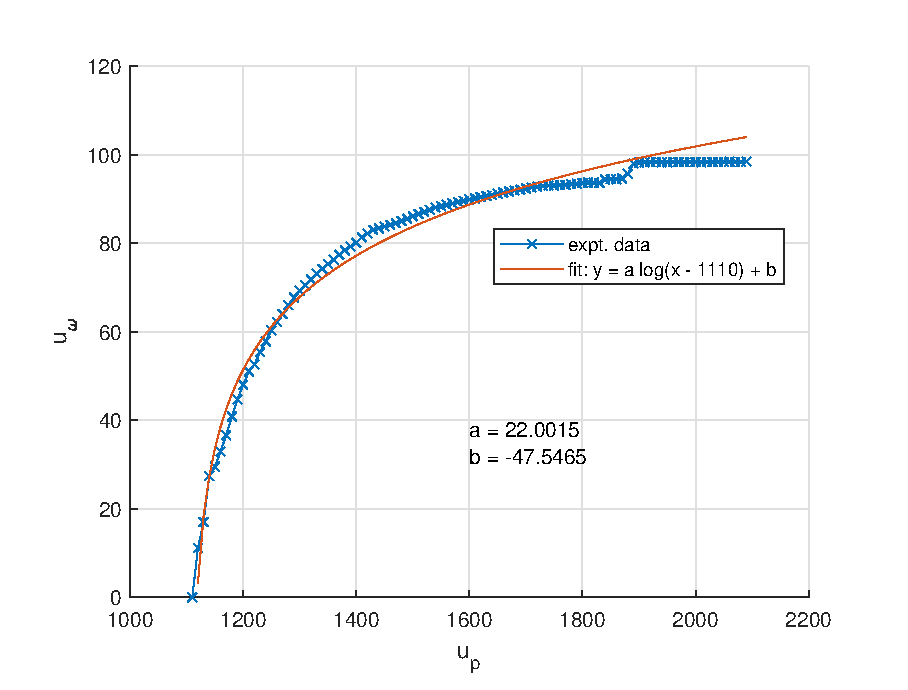
\includegraphics[width = 0.7\textwidth]{./figs/norm_omega/g_w.eps}
    \caption{Logarithmic fit for $g_w()$}
\end{figure}
Thus,
\begin{align*}
    \boxed{g_w(u_p) = 22 \ln(u_p - 1110)- 47.5 }
\end{align*}
and,
\begin{align*}
    g'_w(u_p) = \frac{22}{u_p - 1110}
\end{align*}


\subsubsection{Static mapping with propeller}
Form eqn.~\ref{eqn:prop} and introducing the normalized input from eqn.~\ref{eqn:norm_in}:
\begin{align*}
    J\dot \omega + (K_rK_v + b_f) \omega + C_D \omega^2 + M_f = u K_r V_{in}
\end{align*}

\subsection{Brushless DC motor speed-troque characteristics \cite{crowder2019electric}}

The torque and speed characteristics can be determined by the balance between motor's mechanical output power adn electrical input power over a conduction period:
\begin{align*}
    P &= \omega_m T_e = 2 e_p I\\
    e_p &= N_p B_g \pi r l \omega_m\\
    \text{Where, } \qquad &\\
    \omega_m &- \text{Mechanical rpm}\\
    T_e      &- \text{Electromagnetic torque}\\
    e_p      &- \text{Back emf}
\end{align*}

The factor 2 is the result of current flowing through 2-motor phases (trapesoidal wave form).\\

We have, electromagnetic torque:
\begin{align*}
    T_e &= 4 N_p B_g l r I &[\because \text{Lenz law}]
\end{align*}
let, $E = 2 e_p$. We have,
\begin{align*}
    E &= k \psi \omega_m = K_v \omega_m\\
    T_e &= k \psi I = K_T I\\
\text{Where, } \qquad &\\
    k &= 4 N_p  &(\text{Armature Constant})\\
    \psi &= B_g \pi  r l  &(\text{Flux})
\end{align*}

Thus, ideally back-emf constant and torque constants are same.\\

Using the above equations, the following steady-state torque speed characteristics can be drived. We have, the instantaneous voltage equation:
\begin{align*}
    V_s &= E + I R\\
\text{Where, } \qquad &\\
    V_s &- \text{Supply voltage}\\
    I &- \text{Total DC current}\\
    R &- \text{Sum of the terminal phase ressistances}
\end{align*}

We have torque speed relationship:
\begin{align*}
    \omega_m &= \omega_0 \left( 1 - \frac{T}{T_0} \right)\\
\text{Where, } \qquad &\\
    \omega_0 &= \frac{V_s}{k \psi} & (\text{No-load Speed})\\
    T_0 &= k \psi I_0              & (\text{Stall Torque})\\
    I_0 &= \frac{V_s}{R}           & (\text{Stall Current})
\end{align*}

\subsection{Dynamic Model (without Propeller)}
We have the dynamic model of BLDC motor using moment balance:
\begin{align*}
    J_m \dot \omega_m &= T_e - b_f \omega_m - M_f\\
    \text{where, } \qquad &\\
    J_m &- \text{Moment of inertia of the motor}\\
    b_f &- \text{lumped parameter for viscous friction}\\
    M_f &- \text{lumped parameter for coulomb friction}
\end{align*}
\itbf{Friction:}
\begin{enumerate}
    \item Viscous friction: $-b_f \omega$.
    \item Columb friction: $-M_{f} \sign(\omega) = -M_{f} \qquad [\because$ the motor turns in only one direction $]$.
\end{enumerate}

\medskip

From the speed-torque characteristics of the BLDC motor:
\begin{align*}
    T_e &= K_T I = K_T \frac{(V_s - E)}{R} = \frac{K_T}{R} (V_s - K_v \omega_m)  & [\because K_v = K_T = k \psi]\\
    \text{Let, }\qquad \qquad &\\
    K_r &= \frac{K_T}{R}
\end{align*}
From the definition of Input to ESC:
\begin{align*}
    V_s &= u V_{in}\\
    \therefore T_e &= u K_r V_{in} - K_r K_v \omega_m
\end{align*}

Substituting:
\begin{align*}
    &J_m \dot \omega_m = u K_r V_{in}  - K_rK_v \omega_m  - b_f \omega_m - M_f
\end{align*}
\begin{equation}
    \boxed{
    J_m \dot \omega_m + (K_r K_v  + b_f) \omega_m + M_f = u K_r V_{in}
    }
\end{equation}

\subsection{BLDC Motor with Propeller}
Adding propeller moment of inertia and the moment due to propeller drag into the BLDC motor model.
\begin{align*}
    (J_m + J_p) \dot \omega + (K_rK_v + b_f) \omega + M_f &= u K_r V_{in} - C_D \omega^2
\end{align*}
Where, $C_D$ is the aerodynamic drag. Let, $J_m + J_p = J$
\begin{equation}
    \boxed{
    J\dot \omega + (K_rK_v + b_f) \omega + C_D \omega^2 + M_f = u K_r V_{in}
    }
\end{equation}


%    \text{Substituting, } \quad K_r u &= (K_r K_v  + b_f) u_\omega + \frac{M_f}{\hat V_{in}}\\
%   J\dot \omega + (K_rK_v + b_f) \omega + C_D \omega^2 + M_f &= V_{in} \left((K_r K_v  + b_f) u_\omega + \frac{M_f}{\hat V_{in}} \right)\\



% \begin{align*}
%     \text{Using normalized no-load angular velocity input:} &\\
%     J_m \dot \omega_m + (K_r K_v  + b_f) \omega_m + M_f &= \left(\left(\frac{K_r K_v  + b_f}{K_r} \right) u_{\omega} + \frac{M_f}{K_r \hat V_{in}} \right) K_r V_{in}\\
%     &= V_{in}(K_r K_v  + b_f)u_{\omega} + M_f \frac{V_{in}}{\hat V_{in}}
% \end{align*}

% We get the linearised model using small perturbtation:
% \begin{align*}
%     J_m \delta \dot \omega_m + (K_rK_v + b_f) \delta  \omega_m  &= \delta u_{\omega}V_{in}(K_r K_v  + b_f) \\
%     \frac{\delta \omega_m (s)}{\delta u (s)} &= \frac{V_{in}(K_r K_v  + b_f)}{J_m s + (K_r K_v + b_f)} = \frac{V_{in}}{\frac{J_m}{(K_r K_v + b_f)} s + 1} = \frac{K_m}{\tau_m s + 1}\\
%     \text{where, }\qquad &\\
%     K_m &= V_{in}\\
%     \tau_m &= \frac{J_m}{(K_rK_v + b_f)}
% \end{align*}

% \begin{minipage}{0.49\textwidth}
% Writing interms of $\delta u_p$:
% \begin{align*}
%    \delta u_\omega &= g'_w(u_p) \delta u_p\\
%    \implies \frac{\delta \omega_m (s)}{\delta u_{p} (s)} &= \frac{K g'_w(u_p)}{\tau s + 1}
% \end{align*}
% This explains the static gain variation observed in the system identification.
% \end{minipage}
% \begin{minipage}{0.49\textwidth}
%  \begin{figure}[H]
%     \centering
%     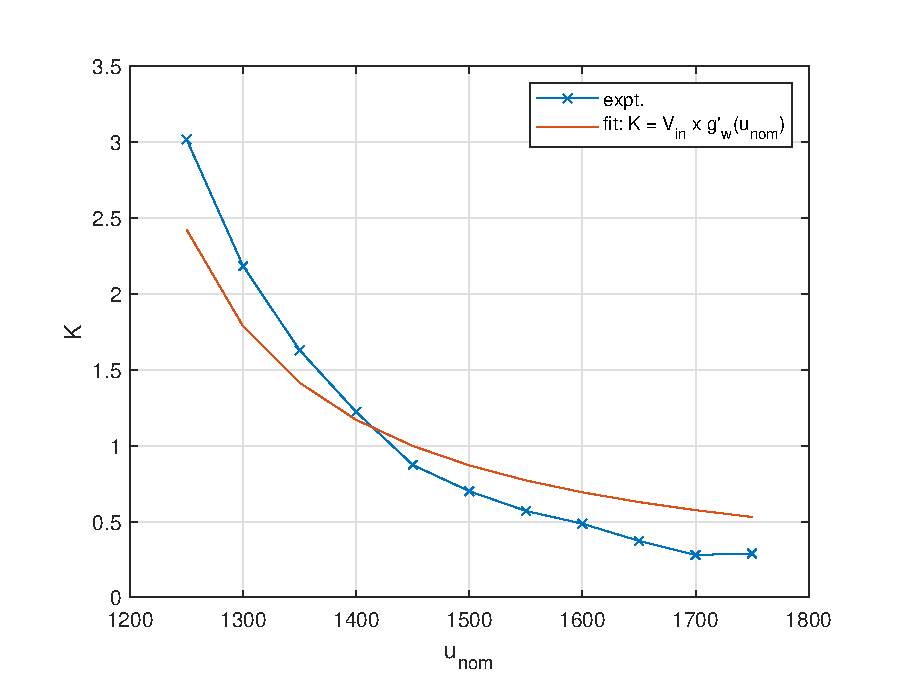
\includegraphics[width = \textwidth]{./figs/norm_omega/K_fit.eps}
%     \caption{Static gain variation with nominal input ($u_p$) with input perturbtation $\delta u_p = 100 \mu s$}
% \end{figure}
% \end{minipage}
% %===============================================================================
%\subsection{Parametric Identification model for BLDC motor dyanmcis}
%\subsubsection{Continuous Parametric Model}
%\begin{align*}
%    J_m \dot \omega &= -(K_rK_v + b_f) \omega_m - M_f + u K_r V_{in}\\
%   %===
%    \implies \dot \omega &= -\frac{(K_rK_v + b_f)}{J_m} \omega_m - \frac{M_f}{J_m} + u \frac{K_r V_{in}}{J_m}
%\end{align*}
%
%Hence, we have the continuous parametric model:
%$$ \dot \omega =
%    \underbrace{\begin{bmatrix}
%               - \omega  & -1
%\end{bmatrix}}_{\Phi^T(\omega)}
%\underbrace{\begin{bmatrix}
%    \frac{(K_rK_v + b_f)}{J_m}  \\
%    \frac{M_f}{J_m}
%\end{bmatrix} }_{\pmb \theta}
%    +\frac{K_r V_{in}}{J_m}u $$
%
%Let,
%\begin{align*}
%    a_1 &= \frac{(K_rK_v + b_f)}{J_m} \qquad
%    a_2 =   \frac{M_f}{J_m}\\
%    \\
%    \pmb \theta &= \begin{bmatrix}a_1 & a_2 \end{bmatrix}^T \qquad
%    b =  \frac{K_r V_{in}}{J_m}
%\end{align*}
%
%$$\therefore \dot \omega = \Phi^T(\omega) \pmb \theta + b u$$
%
%\subsubsection{Descritezed Parametric Model}
%Descritizing the above model using euler-method $\left(\dot \omega = \frac{\omega[k] - \omega[k-1]}{h}\right)$, with $h$ as the sampling interval:
%
%\begin{align*}
%    \frac{\omega[k] - \omega[k-1]}{h} &=
%    \begin{bmatrix}  - \omega[k-1]  &  -1 \end{bmatrix}
%    \begin{bmatrix}
%        a_1 \\ a_2
%    \end{bmatrix}
%    + bu[k-1]\\
%    %===
%    \omega[k] &= h \begin{bmatrix} - \omega[k-1]  & -1 \end{bmatrix}
%    \begin{bmatrix}
%        a_1 - \frac{1}{h} \\
%        a_2 \\
%    \end{bmatrix}
%    + b  h u[k-1]\\
%    %===
%    &= h \begin{bmatrix} -\omega[k-1] & -1 & u[k] \end{bmatrix}
%    \begin{bmatrix}
%        a_1 - \frac{1}{h} \\
%        a_2 \\
%        b
%    \end{bmatrix}
%\end{align*}
%
%Let,
%\begin{align*}
%    \pmb \theta_h = h
%    \begin{bmatrix}
%        a_1 - \frac{1}{h} \\
%        a_2 \\
%        b
%    \end{bmatrix} =
%    h
%    \begin{bmatrix}
%        \frac{(K_rK_v + b_f)}{J_m} - \frac{1}{h}  \\
%        \frac{M_f}{J_m}\\
%        \frac{K_r V_{in}}{J_m}
%    \end{bmatrix}
%    \qquad \text{and} \qquad
%    \Phi(\omega[k-1], u[k])^T &=  \begin{bmatrix}  -\omega[k-1] & -1 & u[k-1] \end{bmatrix}
%\end{align*}
%
%hence, we have the parametric model in least-squares form:
%\begin{align*}
%    \omega[k] &= \Phi(\omega[k-1], u[k-1])^T \pmb \theta_h
%\end{align*}
%

%===============================================================================
\newpage
\section{BLDC Motor with Propeller Model}
\subsection{Aerodynamic Model}
\subsection{Propeller Aerodynamics}
Aerodynamics are assumed to be faster than mechanical dynamics of the actuator.
The thrust generation process due to the propagation of pressure wave is assumed to be instantaneous. This assumption is inherent to the standard models that use potential flow theory (lifting-line, blade-element and momentum-disk theories), as they assume incompressible flow.\\

\itbf{Propeller Thrust}:
\begin{align*}
    F_T = C_{T} \omega^2
\end{align*}

\itbf{Propeller moment due to drag}:
\begin{align*}
    M_D = C_{D} \omega^2
\end{align*}

\textbf{Aeroelasticity of the propeller:} It is assumed that the aeroelasticity of the propeller produces high-frequency oscillations in the thrust and torque of the propller which are assumed to be very fast and roll off w.r.t the mechanical dyanmics dyanmics of the actuator as well as the transmission through the propller shaft. The constant  bias in the torque due to flutter is captured in the drag coefficient and it's parameter uncertainity.\\

In the experimental setup, the total moment measured is the result of aerodynamic moment and the friction of the BLDC motor. Thus the total moment becomes:
\begin{align*}
    M = C_D \omega^2 + b_f \omega + M_f
\end{align*}

The aerodynamic coefficients are estimated from the static measuremnts using least-squares estimation.

\begin{align*}
    C_T &= 7.1e-6 \, {N.s^2/rad^2}\\
    C_D &= 2.5e-8 \, {Nm.s^2/rad^2}\\
    b_f &= 9.3e-6 \, {Nm.s/rad}\\
    M_f &= 5.8e-7  \, {Nm}
\end{align*}

\begin{figure}[H]
    \begin{minipage}{0.49\textwidth}
        \begin{figure}[H]
            \centering
            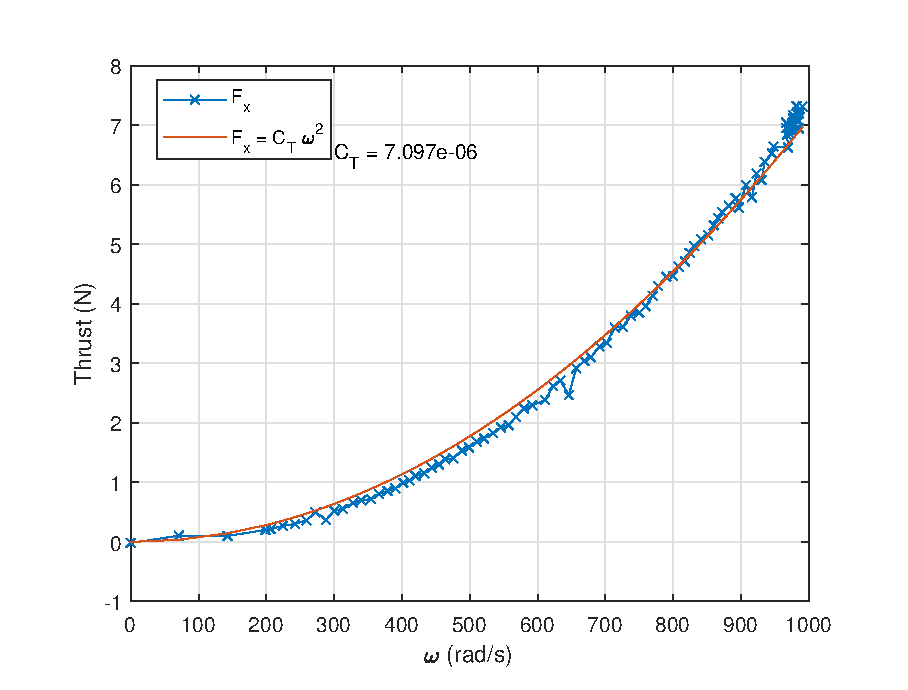
\includegraphics[width = \textwidth]{./figs/aero/Fx.eps}
        \end{figure}
        \caption{Variation of thrust with rpm}
    \end{minipage}
    \begin{minipage}{0.49\textwidth}
        \begin{figure}[H]
            \centering
            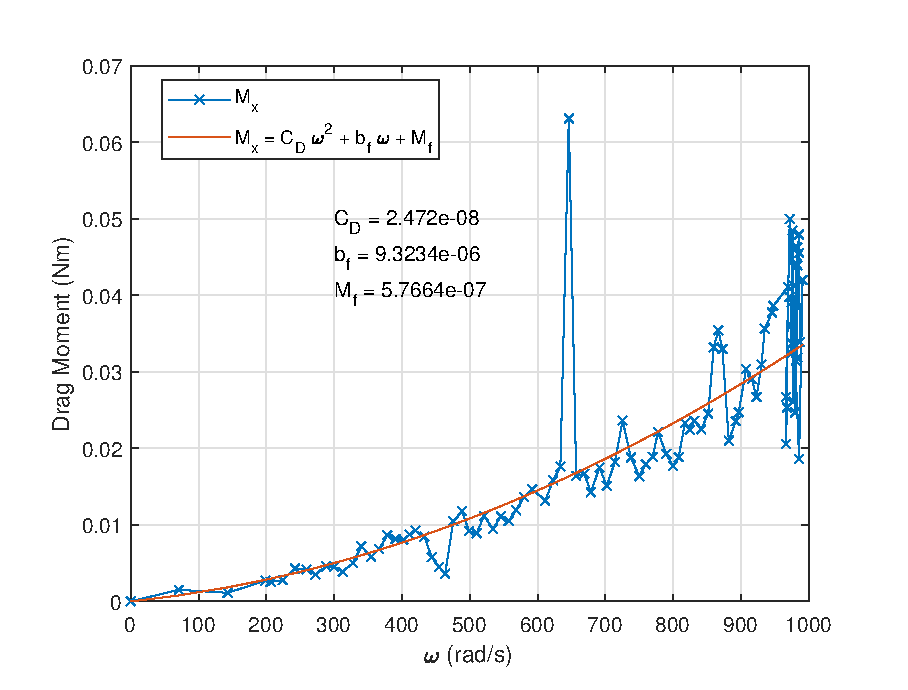
\includegraphics[width = \textwidth]{./figs/aero/Mx.eps}
            \caption{Variation of drag moment with rpm}
        \end{figure}
    \end{minipage}
\end{figure}


We get the linearised model using small perturbtation:
\begin{align*}
     J \delta \dot \omega + (K_r K_v + b_f) \delta \omega + 2 C_D \omega_0 \delta \omega  &= \delta u_\omega (K_r K_v  + b_f)  V_{in}\\
    J \delta \dot \omega + (K_r K_v + b_f + 2 C_D \omega_0) \delta \omega  &=\delta u_\omega (K_r K_v  + b_f)  V_{in}
\end{align*}
Thus we have the trannsfer function model:
\begin{align*}
    \frac{\delta \omega(s)}{\delta u_\omega (s)} &=
    \frac{(K_r K_v  + b_f)  V_{in}}{J s + (K_rK_v + b_f + 2 C_D \omega_0)} = \frac{\frac{V_{in}}{\left(1 + \frac{2 C_D}{K_r K_v + b_f} \omega_0 \right)}}{\frac{J}{(K_r K_v + b_f + 2 C_D \omega_0)}s + 1} = \frac{K_p}{\tau_p s + 1}\\
    \text{Where, }\qquad &\\
    K_p &= \frac{K_r K_v + b_f}{(K_rK_v + b_f + 2 C_D \omega_0)} V_{in}\\
    \tau_p &= \frac{J}{(K_rK_v + b_f + 2 C_D \omega_0)}
\end{align*}

Thus both gain and time-constant vary with the nominal rpm. Effectively, the cutoff frequency is the only parameter that varies with nominal rpm. When the above trannsfer function is written in the form:
\begin{align*}
    \frac{\delta \omega(s)}{\delta u_w(s)} &= \frac{k_p}{s + \omega_p} = \frac{\frac{(K_rK_v + b_f) V_{in}}{J}}{s + \frac{(K_rK_v + b_f + 2 C_D \omega_0)}{J}}\\
    \text{Where, } \qquad &\\
    k_p &= \frac{(K_rK_v + b_f) V_{in}}{J} & (\text{Independent of } \omega_0)\\
    \omega_p &= \frac{(K_rK_v + b_f + 2 C_D \omega_0)}{J}
\end{align*}

This information will be used for establishing the validity of identified model.

In case of using $u_p$ as input:
\begin{align*}
    \frac{\delta \omega(s)}{\delta u_p(s)} &= \frac{g'_w (u_p) k_p}{s + \omega_p} = \frac{\left(\frac{22 k_p}{u_p - 1110}\right)}{s + \omega_p}
\end{align*}

Thus in this case the numerator gain varies inversely with $u_{p_{nom}}$ and $\omega_p$ varies with $\omega_0$.

%===============================================================================
\subsection{Parametric Identification model for BLDC motor - propeller dyanmcis}
Let, $J$ be the total moment on inertia along the normal axis. Then,
\begin{align*}
    J \dot \omega &= -(K_rK_v + b_f) \omega_m - M_f - C_D \omega_m^2 + u K_r V_{in}\\
   %===
    \implies J\dot \omega &= -(K_rK_v + b_f) \omega - C_D \omega^2 - M_f + V_{in} \left((K_r K_v  + b_f) u_\omega + \frac{M_f}{\hat V_{in}} \right)\\
   %===
        &= -(K_rK_v + b_f) \omega - C_D \omega^2 - M_f \left( 1 - \frac{V_{in}}{\hat V_{in}}\right) + V_{in} \left((K_r K_v  + b_f) u_\omega  \right)\\
    %==
    \implies J \dot \omega &= -(K_rK_v + b_f)\omega_m - C_D \omega_m^2 - M_f \left( 1 - \frac{V_{in}}{\hat V_{in}}\right) + u_\omega (K_rK_v + b_f) V_{in}
    %===
\end{align*}
$$\boxed{J \dot \omega + (K_rK_v + b_f)\omega + C_D \omega_m^2 + M_f \left( 1 - \frac{V_{in}}{\hat V_{in}}\right) =  u_\omega (K_rK_v + b_f) V_{in}}$$

As $M_m = (K_rK_v + b_f) \omega + C_D \omega^2 + M_f \left( 1 - \frac{V_{in}}{\hat V_{in}}\right) $ is measured, we use it in the right-hand side of parameter esitmation to reduce the number of parameters.

Descritizing the above equation:
\begin{align*}
    \frac{J}{h} (\omega[k+1] - \omega[k]) - u_\omega[k] (K_rK_v + b_f) V_{in} &= - M_m \\
    %===
    J(\omega[k+1] - \omega[k]) - u_\omega[k] h(K_rK_v + b_f) V_{in} &= - M_m h \\
    %===
    \underbrace{\bm{(\omega[k+1] - \omega[k]) & -h u_\omega[k]} }_{\phi(\omega[k+1], \omega[k], u[k])} \underbrace{\bm{J \\ (K_rK_v + b_f) V_{in} }}_{\pmb \theta} &= - M_m h
\end{align*}



% Hence, we have the continuous parametric model:
% $$ \dot \omega =
%     \underbrace{\begin{bmatrix}
%     - \omega^2 & - \omega  & -1
% \end{bmatrix}}_{\Phi^T(\omega)}
% \underbrace{\begin{bmatrix}
%     \frac{C_{D}}{J} \\
%     \frac{(K_rK_v + b_f)}{J}  \\
%     M_f \left( 1 - \frac{V_{in}}{\hat V_{in}}\right)
% \end{bmatrix} }_{\pmb \theta}
%     +\left(\frac{(K_rK_v + b_f)}{J} V_{in}\right) u_{\omega}
%  $$

% Let,
% \begin{align*}
%     a_1 = \frac{C_{D}}{J}  \qquad
%     a_2 &= \frac{(K_rK_v + b_f)}{J} \qquad
%     a_3 =   M_f \left( 1 - \frac{V_{in}}{\hat V_{in}}\right)\\
%     \\
%     \pmb \theta = \begin{bmatrix}a_1 & a_2 & a_3 \end{bmatrix}^T &\qquad
%     b = \frac{(K_rK_v + b_f)}{J} V_{in} = a_2 V_{in}
% \end{align*}

% $$\therefore \dot \omega = \Phi^T(\omega) \pmb \theta + b u$$

% \subsubsection{Descritezed Parametric Model}
% Descritizing the above model using euler-method $\left(\dot \omega = \frac{\omega[k] - \omega[k-1]}{h}\right)$, with $h$ as the sampling interval:

% \begin{align*}
%     \frac{\omega[k] - \omega[k-1]}{h} &=
%     \begin{bmatrix} - \omega^2[k-1] & - \omega[k-1]  &  -1 \end{bmatrix}
%     \begin{bmatrix}
%         a_1 \\ a_2 \\ a_3
%     \end{bmatrix}
%     + bu[k-1]\\
%     %===
%     \omega[k] &= h \begin{bmatrix} - \omega^2[k-1] & - \omega[k-1]  & -1 \end{bmatrix}
%     \begin{bmatrix}
%         a_1 \\
%         a_2 - \frac{1}{h} \\
%         a_3 \\
%     \end{bmatrix}
%     + b  h u[k-1]\\
%     %===
%     &= h \begin{bmatrix} - \omega^2[k-1] & -\omega[k-1] & -1 & u[k] \end{bmatrix}
%     \begin{bmatrix}
%         a_1 \\
%         a_2 - \frac{1}{h} \\
%         a_3 \\
%         b
%     \end{bmatrix}
% \end{align*}

% Let,
% \begin{align*}
%     \pmb \theta_h = h
%     \begin{bmatrix}
%         a_1 \\
%         a_2 - \frac{1}{h} \\
%         a_3 \\
%         b
%     \end{bmatrix} =
%     h
%     \begin{bmatrix}
%         \frac{C_{D}}{J} \\
%         \frac{(K_rK_v + b_f)}{J} - \frac{1}{h}  \\
%         M_f \left( 1 - \frac{V_{in}}{\hat V_{in}}\right)\\
%         \frac{(K_rK_v + b_f)}{J} V_{in}
%     \end{bmatrix}
%     \qquad \text{and} \qquad
%     \Phi(\omega[k-1], u[k])^T &=  \begin{bmatrix} - \omega^2[k-1] & -\omega[k-1] & -1 & u[k-1] \end{bmatrix}
% \end{align*}

% hence, we have the parametric model in least-squares form:
% \begin{align*}
%     \omega[k] &= \Phi(\omega[k-1], u[k-1])^T \pmb \theta_h
% \end{align*}

%\subsubsection{Input singal (persistance of exitation and frequency limitation)}
%\textbf{Note:}
%\begin{enumerate}
%    \item PE order of a square wave of half-period m is m+1.
%    \item PE order of a single sine wave is 2.
%\end{enumerate}
%Hence, a sum of sinusoids wave with atleast 3 waves within the frequency of 45 Hz (the limitation is due to the structure) can be used to estimate the parameters and the coefficients of force and torque generated.
%

%===============================================================================
\newpage
\section{Dynamic Model Parameter Identification}
\subsection{BLDC Motor}
\subsection{BLDC Motor and Propeller}
%===============================================================================
\newpage
\section{Conclusion: Model and Model Parameters}
\subsection{Parametric Form}
%===============================================================================
%\newpage
%\section{Gyroscopic Effects of Propeller Inertia}
%===============================================================================
\bibliographystyle{unsrt}
\bibliography{refs}

\end{document}
